% Template for ICIP-2009 paper; to be used with:
%          spconf.sty  - ICASSP/ICIP LaTeX style file, and
%          IEEEbib.bst - IEEE bibliography style file.
% --------------------------------------------------------------------------
\documentclass{article}
\usepackage{spconf,amsmath,epsfig,subfig,graphicx,algorithm,algorithmic,subfig}

% Example definitions.
% --------------------
\def\x{{\mathbf x}}
\def\L{{\cal L}}

% Title.
% ------
\title{AUTHOR GUIDELINES FOR ICIP 2009 PROCEEDINGS MANUSCRIPTS}
%
% Single address.
% ---------------
\name{Author(s) Name(s)\thanks{Thanks to XYZ agency for funding.}}
\address{Author Affiliation(s)}
%
% For example:
% ------------
%\address{School\\
%	Department\\
%	Address}
%
% Two addresses (uncomment and modify for two-address case).
% ----------------------------------------------------------
%\twoauthors
%  {A. Author-one, B. Author-two\sthanks{Thanks to XYZ agency for funding.}}
%	{School A-B\\
%	Department A-B\\
%	Address A-B}
%  {C. Author-three, D. Author-four\sthanks{The fourth author performed the work
%	while at ...}}
%	{School C-D\\
%	Department C-D\\
%	Address C-D}
%
\begin{document}
%\ninept
%
\maketitle
%
\begin{abstract}
Abstract goes here
\end{abstract}
%
\begin{keywords}
One, two, three, four, five
\end{keywords}
%
\section{Introduction}
\label{sec:intro}
Intro

\section{Prior Research}
\label{sec:prior}
Prior Work

\section{Methodology}
\label{sec:methodology}

\subsection{Image Enhancement}
The acquired Bayer array images are reconstructed into their RGB representation and then converted to grayscale. This is followed by a temporal blurring process which helps to connect the dashed lane marker sequence in the image serving as an enhancement stage \cite{borkar_layered_2009}.

\subsection{Inverse Perspective Mapping}
%\begin{figure}[htb]
%  \centering
%  \subfloat[Extracted ROI]{\label{fig:temp_blur_before}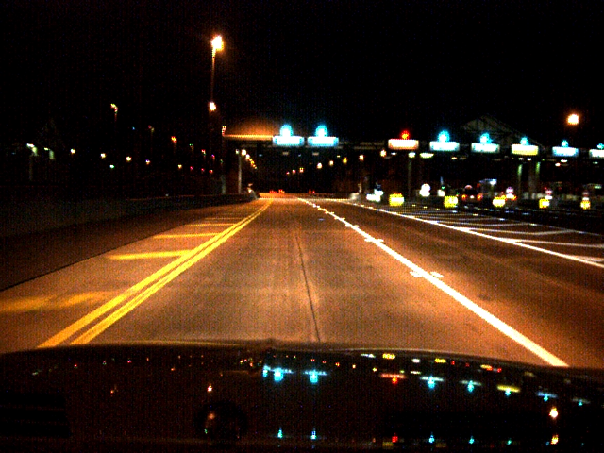
\includegraphics[width=0.2655\textwidth]{IMG/fwd_camera_view.png}}\hspace{0.001in}
%  \subfloat[ROI with temporal blur]{\label{fig:temp_blur_after}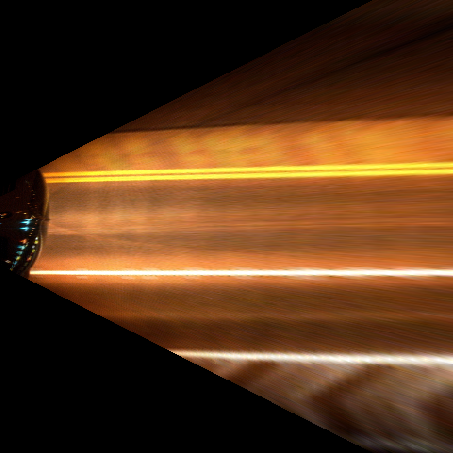
\includegraphics[width=0.20\textwidth]{IMG/ipm_image_color.png}}
%  \caption{Intermediate results of the temporal blur}
%  \label{fig:temp_blur}
%\end{figure}
Inverse perspective mapping (IPM) is an image transformation technique used to remove the perspective effect from an image. Application of this transform changes the appearance of the image from a forward facing camera view to a birds eye view \cite{sehestedt_robust_2007,shu_vision_2004,bertozzi_gold:parallel_1998}. The benefit of this approach is the simplification of lane marker detection and classification as the initially converging lane marker sequences now appear parallel. In addition, the transformation enables a mapping between pixels in the image plane to their corresponding locations in the world with metric co-ordinates. Camera parameters such as height from the ground, inclination and horizontal/vertical viewing angles need to be determined ahead of time to guarantee an accurate transformation. The IPM transform is applied to the average image acquired after application of the enhancements above.

\subsection{Lane Candidate Location Detection}
An adaptive threshold is applied to the IPM average image to generate a binary image which it is split into two halves \cite{borkar_layered_2009}. A low resolution Hough transform is then computed on the binary images and a set of X highest scoring lines are formulated into a list for each half image \cite{borkar_layered_2009}. Each line in the list is then sampled along its length at specific distance co-ordinates. The corresponding location of each of these points in the IPM average image is recovered. A 1-D search window centered at each point in the IPM average image is used in the matched filter. With the birds eye view, the visualization of the lane marker sequence not only appears parallel, but each lane marker also maintains a constant width in the entire image; consequently, a fixed size and fixed variance Gaussian kernel is used in the matched filter. This was not the case in \cite{borkar_layered_2009} where a variety of variances had to be used to create the kernel on different scanlines. Matched filtering is iteratively performed on the remaining X-1 lines. As each of the X lines is sampled at the specific co-ordinates, X filtering results are available at each of these positions upon completing the iterations. As a result, the location with the highest correlation coefficient at each distance co-ordinate is chosen as the best estimate.

Upon acquiring the sequence of best estimates, Random Sample Consensus (RANSAC) is applied to the data points. The generic RANSAC algorithm robustly fits a model through the most probable data set or inliers while rejecting outliers \cite{hartley_multiple_2004,fischler_random_1981}. Linear Least Squares Estimation (LSE) is then used to fit to a line on the inliers. The orientation of line modeled in terms of $\rho$ and $\theta$ with respect to the origin of the image (top left). For data fitting, a line was chosen over a parabolic fit since the latter is more sensitive to minor perturbations in the inliers resulting many times in unacceptable outcomes.\\
\subsection{Tracking}
The orientation of the fitted line is predicted using a Kalman filter. The state vector $x(n)$ and observation vector $y(n)$ are defined as
\begin{equation}
x(n)= y(n)=\begin{bmatrix} \rho\\\dot{\rho}\\\theta\\\dot{\theta} \end{bmatrix}\\
\label{eq:state_measure_vectors}
\end{equation}\\
where $\rho$ and $\theta$ are variables modeling the orientation of the line while $\dot{\rho}$ and $\dot{\theta}$ represent the derivatives of $\rho$ and $\theta$ computed over the current and previous frames. Piece-wise linearity is assumed between the frames allowing use of the Kalman filter. The state transition matrix $A$ and observation model $C$ are define as
\begin{equation}
A = \begin{bmatrix} 1 && 1 && 0 && 0 \\ 0 && 1 && 0 && 0 \\ 0 && 0 && 1 && 1 \\ 0 && 0 && 0 && 1 \\\end{bmatrix}\\
\label{eq:state_trans}
\end{equation}\\
\begin{equation}
C = \begin{bmatrix} 1 && 0 && 0 && 0 \\ 0 && 1 && 0 && 0 \\ 0 && 0 && 1 && 0 \\ 0 && 0 && 0 && 1 \\\end{bmatrix}\\
\label{eq:observation_model}
\end{equation}\\
The independence between the variables in $x(n)$ and $y(n)$ allows creation of simple covariance matrices $Q_w$ and $Q_v$. $Q_w$ and $Q_v$ represent the process and observation noise respectively. 
\begin{algorithm}[htb]
\caption{Kalman filter implementation}
\label{algo:Kalman_Implementation}
\begin{algorithmic}[1]
\FOR{($n$=Current Frame)}
\STATE $\hat{x}(n|n-1)=A(n-1)\hat{x}(n-1|n-1)$
\STATE $P(n|n-1)=A(n-1)P(n-1|n-1)A^H(n-1)+Q_w(n)$
\STATE $K(n)=P(n-1|n-1)C^H(n)[C(n)P(n|n-1)C^H(n)+Q_v(n)]^{-1}$
\STATE $\hat{x}(n|n)=\hat{x}(n|n-1)+K(n)[y(n)-C(n)\hat{x}(n|n-1)]$
\STATE $P(n|n)=[I-K(n)C(n)]P(n|n-1)$
\ENDFOR
\end{algorithmic}
\end{algorithm}
The covariance matrices are defined as identity and multiplied with non-uniform weights along the diagonal, these weights correspond to the variances of the parameters in $x(n)$ and $y(n)$. As measurements tends to be noisy, the Kalman filter acts like low-pass filter by smoothing the observed values. In algorithm \ref{algo:Kalman_Implementation}, the Kalman filter recursively predicts the state vector from the previous available information. $P(n)$ and $K(n)$ represent error covariance matrix and optimal Kalman gain.

In the case of a lane marker sequence not being detected, the values in $Q_v$ are increased significantly and $\hat{x}(n|n)$ is modified as Eq. \ref{eq:xnn_mod} 
\begin{equation}
\hat{x}(n|n) = \hat{x}(n|n-1)
\label{eq:xnn_mod}
\end{equation}\\
to force the Kalman filter to rely purely on prediction. After extraction from $\hat{x}(n|n)$, $\rho$ and $\theta$ are transformed back to the image plane and used to model the estimated orientation of the lane marker sequence. The series of iterated matched filtering and tracking is similarly performed on the other half image.

\section{Results}
\label{sec:results}

\section{Conclusions}
\label{sec:concl}


\section{Future Work}
\label{sec:print}

%\vfill
%\pagebreak

% References should be produced using the bibtex program from suitable
% BiBTeX files (here: strings, refs, manuals). The IEEEbib.bst bibliography
% style file from IEEE produces unsorted bibliography list.
% -------------------------------------------------------------------------
\bibliographystyle{IEEEbib}
\bibliography{refs}

\end{document}
